% This is "sig-alternate.tex" V2.1 April 2013
% This file should be compiled with V2.5 of "sig-alternate.cls" May 2012
%
% This example file demonstrates the use of the 'sig-alternate.cls'
% V2.5 LaTeX2e document class file. It is for those submitting
% articles to ACM Conference Proceedings WHO DO NOT WISH TO
% STRICTLY ADHERE TO THE SIGS (PUBS-BOARD-ENDORSED) STYLE.
% The 'sig-alternate.cls' file will produce a similar-looking,
% albeit, 'tighter' paper resulting in, invariably, fewer pages.
%
% ----------------------------------------------------------------------------------------------------------------
% This .tex file (and associated .cls V2.5) produces:
%       1) The Permission Statement
%       2) The Conference (location) Info information
%       3) The Copyright Line with ACM data
%       4) NO page numbers
%
% as against the acm_proc_article-sp.cls file which
% DOES NOT produce 1) thru' 3) above.
%
% Using 'sig-alternate.cls' you have control, however, from within
% the source .tex file, over both the CopyrightYear
% (defaulted to 200X) and the ACM Copyright Data
% (defaulted to X-XXXXX-XX-X/XX/XX).
% e.g.
% \CopyrightYear{2007} will cause 2007 to appear in the copyright line.
% \crdata{0-12345-67-8/90/12} will cause 0-12345-67-8/90/12 to appear in the copyright line.
%
% ---------------------------------------------------------------------------------------------------------------
% This .tex source is an example which *does* use
% the .bib file (from which the .bbl file % is produced).
% REMEMBER HOWEVER: After having produced the .bbl file,
% and prior to final submission, you *NEED* to 'insert'
% your .bbl file into your source .tex file so as to provide
% ONE 'self-contained' source file.
%
% ================= IF YOU HAVE QUESTIONS =======================
% Questions regarding the SIGS styles, SIGS policies and
% procedures, Conferences etc. should be sent to
% Adrienne Griscti (griscti@acm.org)
%
% Technical questions _only_ to
% Gerald Murray (murray@hq.acm.org)
% ===============================================================
%
% For tracking purposes - this is V2.0 - May 2012
\documentclass{sig-alternate-05-2015}
\usepackage{booktabs}
\usepackage{subcaption}
\usepackage[english]{babel}
\usepackage{graphicx}
\usepackage{epstopdf}
\usepackage{tabularx}


\begin{document}
	\begingroup
	\onecolumn
	\setlength{\unitlength}{1cm}
	\center
	\large
	
	\begin{picture}(12.0, 2)
	\put(0.1, 0){
\includegraphics[draft=false,height=1.5cm]{uctlogo}}
	\put(10.7, 0.1){
\includegraphics[draft=false,height=1.3cm]{cslogo}}
	\end{picture}
	\\
	\vspace{0.3cm}
	\textsc{ \Large
		Department of Computer Science
	}
	
	\vspace{1cm}
	
	\textsc{ \huge
		Computer Science Honours \\
		Final Paper \\
		2016 \\
	}
	
	\vspace{1cm}
	
	\renewcommand{\arraystretch}{2}
	\begin{tabularx}{0.8\textwidth}{l@{\hspace{1cm}}X}
		Title: &
		An Analysis of Classification Techniques for the Prediction of Tuberculosis Defaulters and Community Health Worker Attrition \\
		Author: &
		Brian Mc George \\
		Project abbreviation: &
		\textsc{ML4CHW} \\
		Supervisor: &
		Dr Brian DeRenzi
	\end{tabularx}
	
	\vspace{3cm}
	
	\renewcommand{\arraystretch}{1.25}
	\begin{tabular}{|l|c|c|c|}
		\hline
		\textbf{Category} & \textbf{Min} & \textbf{Max} & \textbf{Chosen} \\ \hline \hline
		Requirement Analysis and Design & 0 & 20 &
		 \\ \hline
		Theoretical Analysis & 0 & 25 &
		 \\ \hline
		Experiment Design and Execution & 0 & 20 &
		19 \\ \hline
		System Development and Implementation & 0 & 15 &
		10 \\ \hline
		Results, Findings and Conclusion & 10 & 20 &
		18 \\ \hline
		Aim Formulation and Background Work & 10 & 15 &
		13 \\ \hline
		Quality of Paper Writing and Presentation & \multicolumn{2}{c|}{10} &
		10 \\ \hline
		Quality of Deliverables & \multicolumn{2}{c|}{10} &
		10 \\ \hline
		Overall General Project Evaluation & 0 & 10 &
		\\ \hline
		\hline
		\multicolumn{3}{|l|}{\textbf{Total marks}} & 80 \\ \hline
	\end{tabular}
	
	\endgroup
	\thispagestyle{empty}
	\newpage
	\setcounter{page}{1}
	
	
	% Copyright
	\setcopyright{acmcopyright}
	%\setcopyright{acmlicensed}
	%\setcopyright{rightsretained}
	%\setcopyright{usgov}
	%\setcopyright{usgovmixed}
	%\setcopyright{cagov}
	%\setcopyright{cagovmixed}
	
	
	% DOI
	\doi{n/a}
	
	% ISBN
	\isbn{n/a}
	
	%Conference
	%\conferenceinfo{PLDI '13}{June 16--19, 2013, Seattle, WA, USA}
	
	%\acmPrice{\$15.00}
	
	%
	% --- Author Metadata here ---
	%\conferenceinfo{WOODSTOCK}{'97 El Paso, Texas USA}
	%\CopyrightYear{2015} % Allows default copyright year (20XX) to be over-ridden - IF NEED BE.
	%\crdata{0-12345-67-8/90/01}  % Allows default copyright data (0-89791-88-6/97/05) to be over-ridden - IF NEED BE.
	% --- End of Author Metadata ---
	
	\title{An Analysis of Classification Techniques for the Prediction of Tuberculosis Defaulters and Community Health Worker Attrition}
	%
	% You need the command \numberofauthors to handle the 'placement
	% and alignment' of the authors beneath the title.
	%
	% For aesthetic reasons, we recommend 'three authors at a time'
	% i.e. three 'name/affiliation blocks' be placed beneath the title.
	%
	% NOTE: You are NOT restricted in how many 'rows' of
	% "name/affiliations" may appear. We just ask that you restrict
	% the number of 'columns' to three.
	%
	% Because of the available 'opening page real-estate'
	% we ask you to refrain from putting more than six authors
	% (two rows with three columns) beneath the article title.
	% More than six makes the first-page appear very cluttered indeed.
	%
	% Use the \alignauthor commands to handle the names
	% and affiliations for an 'aesthetic maximum' of six authors.
	% Add names, affiliations, addresses for
	% the seventh etc. author(s) as the argument for the
	% \additionalauthors command.
	% These 'additional authors' will be output/set for you
	% without further effort on your part as the last section in
	% the body of your article BEFORE References or any Appendices.
	
	%\numberofauthors{8} %  in this sample file, there are a *total*
	% of EIGHT authors. SIX appear on the 'first-page' (for formatting
	% reasons) and the remaining two appear in the \additionalauthors section.
	%
	\author{
		% You can go ahead and credit any number of authors here,
		% e.g. one 'row of three' or two rows (consisting of one row of three
		% and a second row of one, two or three).
		%
		% The command \alignauthor (no curly braces needed) should
		% precede each author name, affiliation/snail-mail address and
		% e-mail address. Additionally, tag each line of
		% affiliation/address with \affaddr, and tag the
		% e-mail address with \email.
		%
		% 1st. author
		\alignauthor
		Brian Mc George\\
		\affaddr{University of Cape Town}\\
		\affaddr{Cape Town, South Africa}\\
		\email{mcgbri004@myuct.ac.za}
	}
	
	\maketitle
	\begin{abstract}
		As the use of electronic data capturing for community health projects becomes more widespread the availability of this type of data for research use is becoming more prevalent. In this paper we outline various issues that may arise when attempting to apply classification techniques to predict minority class events and apply several strategies to counteract them. We focus on the prediction of Tuberculosis defaulters and the attrition of community health workers. We compare 13 classification techniques, 13 data balancing techniques and 6 feature selection techniques to assess what combination produces the best classification results. We find that the use of a data balancing techniques greatly improves balanced accuracy on imbalanced datasets. We recommend the use of Logistic regression, Artificial neural networks, Random Forest and Bernoulli Naive Bayes for different use-cases. Adaptive synthetic sampling is recommended as an over-sampler and edited nearest neighbours as an under-sampler. Random forest is recommended for identifying the most relevant features as well as being able to remove noisy features that do not add to the classification.
	\end{abstract}
	
	%
	%  Use this command to print the description
	%
	\printccsdesc
	
	% We no longer use \terms command
	%\terms{Theory}
	
	%\keywords{ACM proceedings; \LaTeX; text tagging}
	
	\section{Introduction}
	Classification techniques can be used to flag individuals who have a high probability of certain events occurring. In this paper we outline various issues that may arise when attempting to apply classification techniques to predict minority class events and apply several strategies to counteract them. We focus on the prediction of Tuberculosis (TB) defaulters and the attrition of community health workers (CHW).
		
	TB is a global problem and communities often have limited resources to track and follow-up with patients. A patient is considered to have defaulted if their treatment is interrupted for longer than a set duration, typically two months for TB treatment. In 2013 over 210\hspace*{1mm}000 patients defaulted from TB treatment worldwide \cite{world2015TB}. The rate of default in the Americas is the highest at 8\% with Africa at 5\% \cite{world2015TB}. The consequences of defaulting TB treatment include: increased drug resistance, increased health system costs \cite{Lackey:10356751520150601, muture:6660173120110101}, higher risk of mortality, continued risk of transmitting the disease to others \cite{Lackey:10356751520150601} and increased rate of recurrent disease \cite{Jha:10.1371/journal.pone.0008873}. If we can better manage resources towards those patients with a high risk of default then the spread of TB can be reduced. This would also reduce health system costs.
	
	Attrition is the loss of workers through resignation or abandonment of the work. If we can flag workers who are at likely to quit quickly enough then various intervention measures could be implemented in order to retain those workers. This could reduce costs because new workers would not have to be trained.
	
	The aim of this paper is to inform the reader on issues that can occur when building classification models from imbalanced datasets. Bias can occur in the models since most classifiers expect equal weighting of samples for each class. This can lead to poor classification for the minority class, which is often the class of interest. The second aim of this paper is to propose recommendations on classification techniques, data balancing techniques and strategies to improve the overall classification for this problem domain. We examine a number of different data balancing techniques which either over-sample the minority class, under-sample the majority class or provide a combination of an over-sampling and under-sampling technique. We provide a large scale comparison of different classification techniques in order to determine which technique is best suited to these types of problems. As part of our evaluation of each classification technique, we examine how well each classifier works out-of-the-box compared when they are tuned by searching a grid of parameters. Furthermore, we apply a number of feature selection strategies to determine which strategy is best suited to remove redundant and noisy variables.
	
	To facilitate the aforementioned experiments, we developed a testing system which allows new classification techniques and data sets to be supported quickly and easily. The testing system is designed to allow near-exact reproducibility of results.
	
	In addition to our TB default dataset and attrition dataset, we include two real-world credit scoring datasets. The field of credit scoring in the financial space aims to determine if a financial institution should provide credit to an individual. This is a well researched binary classification problem. We included these as all the problems try to flag high-risk individuals and it will allow us to get a better understanding of how the results compare and generalise.
	
	From our findings we recommend the use of Logistic regression (LR), Artificial neural networks (ANN), Random Forest (RF) and Bernoulli Naive Bayes (NB) for different use-cases. All the classifiers produced good classification results. LR is recommended when it is important to be able to understand how the model is producing the classification. ANN and RF are recommended when raw classification performance is the main concern. Bernoulli NB scales well with dataset size and requires very little tuning making it ideal for rapid testing and iteration on one's experimental design. Adaptive synthetic sampling is recommended as an over-sampler and edited nearest neighbours as an under-sampler. RF is recommended for identifying the most relevant features as well as being able to remove noisy features that do not add to the classification.
	
	\section{Background}
	This section aims to provide an overview of all the techniques and metrics used in this paper.
	\subsection{Definition of a defaulter}
	The definition of a defaulter depends on its context. TB literature typically uses the World Health Organisation (WHO) definition that a defaulter is a person whose treatment has been disrupted for two or more consecutive months \cite{chan:2003prevalence, cherkaoui:19326203, Jha:10.1371/journal.pone.0008873,jittimanee:10.1111/j.1440-172X.2007.00650.x,muture:6660173120110101, world2015TB}.
	
	\subsection{Classification techniques}
	We selected a variety of classification techniques to benchmark. We include a selection of well known techniques, ensemble techniques and newer techniques that have shown promising results in other studies. Our choices are based partly on our review of classification techniques used in the credit scoring field in Section \ref{credit-scoring-review}.
	\subsubsection{Support Vector Machines}
	Support Vector Machines (SVM) maps input vectors into a high-dimensional feature space with the use of a kernel function \cite{Danenas20153194}. The kernel function determines the if the mapping is linear or non-linear \cite{Luo20097562}. Linear, polynomial and radial basis function (RBF) are common kernel functions \cite{hsu2003practical}. The polynomial and RBF kernel performs a non-linear mapping into the high-dimensional space \cite{hsu2003practical}. This feature space is then searched to acquire an optimal hyperplane that separates the space with the maximum distance between the two classes \cite{Danenas20153194}. Hsu \textit{et al.} \cite{hsu2003practical} recommends the RBF kernel as a reasonable first choice but notes that it is not suitable when there are a large number of features. The linear kernel is recommend when there are a large number of features \cite{hsu2003practical}s.
	
	\subsubsection{Artificial Neural Network}
	An ANN is comprised of an input layer, $k$ number of hidden layers and an output layer. Neurons in each layer are connected to the neurons in the next layer. A numeric weight is defined between each pair of connected neurons. An activation function defines if a neuron will fire \cite{Wang2003}. The activation function bounds the value of a neuron to a specific range to limit the effect of divergent neurons \cite{Wang2003}. By using an activation function, a non-linear combination of weights can be generated \cite{Wang2003}. It has been proven that an ANN is able to approximate any continuous function if has at least one hidden node and an activation function that is both bounded to some range and non-constant \cite{Hornik1991251}.
	
	ELM is an alternative approach to the conventional back-propagated ANN. Huang \textit{el al.} \cite{Huang2006489} proved that the input and hidden layer weights can be randomly assigned if the activation function in the hidden layer is infinitely differentiable. By randomly assigning these weights, the weights for the output nodes can be determined analytically \cite{Huang2006489}. This allows ELMs to be trained orders of magnitude faster than a back-propagated ANN \cite{6035797, Huang2006489}. ELMs have been shown to provide better results than SVMs and ANNs on a variety of classification and regression tasks \cite{6035797, Huang2006489}.
	
	\subsubsection{Logistic Regression}
	LR is a technique that models the chance of an outcome based on the input features \cite{doi:10.11613/BM.2014.003}. Since chance is a ratio, the logarithm of the chance is modelled instead \cite{doi:10.11613/BM.2014.003}:
	log$(\frac{p}{1 - p}) = \beta_0 + \beta_1 x_1 + ... + \beta_m x_m$. $p$ represents the probability of an event (likelihood to default for example). $\beta_0$ represents the value of the criterion when the predictor is equal to 0. $\beta_1, ..., \beta_m$ are the regression coefficients associated with the $x_1, ..., x_m$ input features. The probability of an event can then be calculated as $p$ = $\frac{1}{1 + e^{-(\beta_0 + \beta_1 x_1 + ... + \beta_m x_m)}}$. A detailed overview of logistic regression can be found in \cite{Mood01022010} and \cite{doi:10.11613/BM.2014.003}.
	
	\subsubsection{$k$-Nearest Neighbours}
	The $k$-Nearest Neighbours ($k$NN) algorithm determines the output classification by examining the $k$ nearest training examples in the feature space \cite{6313426}. An input is classified by the majority vote of its neighbours.
	
	\subsubsection{Ensembles}
	An ensemble classifier is one which typically makes use of the aggregation of multiple classifiers. A single decision tree (DT) can be used for classification by branching on conjunctions of features and having the leaves represent the output class. A decision tree allows for easy interpretation of the generated model, however, typically provides relatively poor classification accuracy \cite{doi:10.1021/ci034160g}. 
	
	RF is a technique that fits a number of decision trees on random samples with replacement of the dataset. For each tree, $n$ features are randomly selected and the tree is grown \cite{WIDM:WIDM1072}. The output classification is decided by the majority vote of each tree \cite{WIDM:WIDM1072}.
	
	AdaBoost \cite{FREUND1997119} uses a weighted sum of multiple classifiers in order to determine the output. A classifier is constructed in an iterative fashion. At each iteration a pool of classifiers are considered and one classifier is added to the committee of classifiers. Input which is still misclassified is assigned a higher weight at each iteration \cite{Bergstra2006, rojas2009adaboost}. The sign of the function: $C(x) = \sum_{i=1}^{m} \alpha_i k_i$ is used to determine the final classification with $\alpha_i$ denoting the weight of each classifier $k_i$ \cite{Bergstra2006}. 
	
	\subsubsection{Naive Bayes}
	NB makes an assumption that each input feature is independent of each other \cite{Lewis1998, rish2001empirical}. This allows multiple features be uncoupled from one another which simplifies the algorithm. Naive Bayes uses conditional probability to classify new inputs \cite{Lewis1998}. Using Bayes theorem, the following equation is derived: $p(C_i|\textbf{x}) = \frac{p(C_i) \times p(x_1|C_i) \times...\times p(x_n|C_i)}{p(\textbf{x})}$ with input $\textbf{x} = (x_1,...,x_n)$ and class label $C_i$ \cite{Lewis1998, rish2001empirical}. Since $p(\textit{x})$ is identical for each class, it is typically ignored \cite{rish2001empirical}. To classify an input, the probabilities for each class are calculated using the aforementioned equation and the output is the class with the highest probability \cite{Lewis1998}.
	
	The event model of Naive Bayes classification describes the assumed distribution of features. The Gaussian event model assumes that $p(x_i|C_i)$ follows a Gaussian distribution \cite{John:1995:ECD:2074158.2074196}. This allows support of continuous $x_i$ values \cite{John:1995:ECD:2074158.2074196}. The multivariate Bernoulli event model assumes that features are independent boolean values \cite{mccallum1998comparison}.
	
	\subsubsection{Clustering-launched classification}
	Clustering-launched classification (CLC) first clusters the data into groups using a diverse hierarchical k-means algorithm \cite{Luo20097562}. The clusters are divided into positive subsets and negative subsets \cite{Luo20097562}. Support vectors are then used to separate the positive and negative subsets for each cluster \cite{Luo20097562}. Redundant or repeated support vectors are removed thereafter \cite{Luo20097562}.
	
	\subsection{Data Balancing algorithms}
	\label{sec:data_balancing_algorithms}
	This section examines the different data balancing approaches and their respective algorithms. Our problem space often has much fewer samples in the class of interest than the other class. Most classifiers expect an equal number of samples per class otherwise they will bias heavily towards the majority class. we include an analysis of several data balancing algorithms to ensure our classifiers are able to detect both the positive and negative class as best as possible. We chose our balancing techniques to facilitate an evaluation of both over-sampling and under-sampling techniques. Included in the evaluation is techniques that use simple approaches and as others that use sophisticated algorithms.
	\subsubsection{Over-sampling}
	Random over-sampling (ROS) is a technique that randomly replicates examples in the minority class \cite{Batista:2004:SBS:1007730.1007735}. However, this technique can increase the likelihood of over-fitting since exact copies are made from the minority class \cite{Batista:2004:SBS:1007730.1007735}.
	
	The Synthetic minority over-sampling technique (SMOTE) \cite{Chawla:2002:SSM:1622407.1622416} forms new minority samples by interpolating along the line segment on some or all of the $k$ nearest minority class neighbours of a minority example. This approach attempts to alleviate the over-fitting that can occur from using random over-sampling.
	
	Adaptive synthetic sampling (ADASYN) \cite{4633969} is a variation of SMOTE which uses a weighed distribution for different minority class examples according to their difficulty in learning. More synthetic data is generated for minority class examples that are more difficult to learn compared to those that are easier to learn.
	
	\subsubsection{Under-sampling}
	Random under-sampling (RUS) is a technique that randomly eliminates examples in the majority class \cite{Batista:2004:SBS:1007730.1007735}. However, this technique can remove potentially useful information from the training set \cite{Batista:2004:SBS:1007730.1007735}. 
	
	Condensed Nearest Neighbour (CNN) rule \cite{1056066} finds a consistent subset of examples. A subset $D$ of $E$ is consistent if a 1-nearest neighbour classifier trained with $D$ correctly classifies $E$ \cite{Batista:2004:SBS:1007730.1007735}. The process draws one random majority class example and all minority class examples and puts them in $D$ \cite{Batista:2004:SBS:1007730.1007735}. Every misclassified example is then added from $E$ to $D$ \cite{Batista:2004:SBS:1007730.1007735}. This process attempts to remove examples that are far away from the decision border and therefore seen as less relevant for learning \cite{Batista:2004:SBS:1007730.1007735}.
	
	The Tomek link (TL) algorithm \cite{4309452} examines two examples $\textbf{x}_i$ and $\textbf{x}_j$ belonging to different classes. A TL occurs if there is not an example $\textbf{x}_k$ such that $d(\textbf{x}_i, \textbf{x}_k) < d(\textbf{x}_i, \textbf{x}_j)$ or $d(\textbf{x}_j, \textbf{x}_k) < d(\textbf{x}_j, \textbf{x}_i)$. If two examples form a TL then either one is noise or it is a borderline case \cite{Batista:2004:SBS:1007730.1007735}. This information can then be used to under-sample the majority class \cite{Batista:2004:SBS:1007730.1007735}.
	
	One-sided selection (OSS) \cite{Kubat97addressingthe} applies TL to remove borderline and noisy majority class examples then applies CNN to remove majority examples far from the decision border.
	
	Neighbourhood cleaning rule (NCL) \cite{Laurikkala:2001:IID:648155.757340} uses the edited nearest neighbour rule (ENN) to remove majority class examples. ENN removes examples whose label differs from the class of at least two of its nearest 3 neighbours. NCL examines each example $\textbf{x}_i$ and its 3 nearest neighbours. If $\textbf{x}_i$ belongs to the majority class and the neighbours contradict this class then $\textbf{x}_i$ is removed \cite{Batista:2004:SBS:1007730.1007735}. If $\textbf{x}_i$ belongs to the minority class and the neighbours contradict this class then the neighbours from the majority class are removed \cite{Batista:2004:SBS:1007730.1007735}.
	
	Instance threshold hardening (ITH) \cite{Smith:2014:ILA:2843614.2843686} uses the probability estimates from a classifier (such as SVM with a linear kernel) when k-fold cross validation is applied. It selects the $m$ examples from the majority class that have the highest probability estimates for that class when tested in k-fold cross validation. $m$ is the number of samples in the minority class.
	
	NearMiss-1 (NM-1) \cite{mani2003knn} picks majority class examples which have the smallest average distance to the three nearest minority class examples.
	
	Cluster centroids (CC) applies the $k$-means algorithm with $m$ clusters to the majority class and uses the coordinates of the cluster centroids as the majority samples. As in ITH, $m$ is the number of samples in the minority class.	
	
	\subsubsection{Combination}
	SMOTE + TL \cite{batista2003balancing} first applies SMOTE then applies TL. Applying SMOTE can cause minority samples to extend too deep into the majority class space or the opposite where majority class samples extend too deep into the minority class space \cite{batista2003balancing}. TL is used as a data cleaning method to remove examples from both classes to produce well-defined class clusters \cite{batista2003balancing}.
	
	SMOTE + ENN works similarly to SMOTE + TL but ENN is more aggressive at removing samples than TL \cite{Batista:2004:SBS:1007730.1007735}.
	
	\subsection{Evaluation metrics}
	We use a number of metrics to evaluate the performance characteristics of the classifiers and balancing algorithms. Each metric measures a different performance criterion.
	
	The number of true positives (TP), true negatives (TN), false positives (FP) and false negatives (FN) are used to define several metrics which are used to compare the results in this paper. The true positive rate (TPR) or sensitivity defines the proportion of actual positives which are predicted as positive. The TPR is calculated as $\frac{TP}{TP + FN}$. The true negative rate (TNR) or specificity defines the proportion of actual negatives which are predicted as negative. The TNR is calculated as $\frac{TN}{TN + FP}$. 
	
	Accuracy is typically a poor measure of quality for imbalanced datasets as classifiers tend to bias towards the majority class \cite{Batista:2004:SBS:1007730.1007735, Chawla:2004:ESI:1007730.1007733}. Several balanced performance metrics are used instead. Balanced accuracy (BACC) provides an equal weighting in TPR and TNR. It is calculated as $\frac{TPR + TNR}{2}$. Matthews correlation coefficient (MCC) also provides a balanced measure of classification quality and is scored between -1 and 1. The MCC is calculated as: $\frac{(TP \times TN) - (FP \times FN)}{\sqrt{(TP + FP)(TP + FN)(TN + FP)(TN + FN)}}$. 
	
	The Brier score (BS) measures the accuracy of probabilistic predictions in a range of 0 to 1 where a lower score is better \cite{steyerberg2010assessing}. The BS is calculated as: $\frac{1}{N}\sum_{t=1}^{N}(f_t - o_t)^2$ where N is the number of predictions made, $f_t$ is the probability of the positive class being true and $o_t$ is the actual outcome \cite{steyerberg2010assessing}.
	
	The receiver operating curve (ROC) compares TPR for a given FPR. Area under ROC (AUC) is an aggregate measure which averages performance of the classifier over all threshold values. However, recent results suggest that AUC does not treat the relative cost of misclassification the same for each classifier \cite{Hand:2009:MCP:1612990.1613009}. H-measure is an alternative to AUC that remedies this issue through use of a $\beta$-distribution which specifies the relative severity of misclassification in a consistent manner for each classifier \cite{Hand:2009:MCP:1612990.1613009}. H-measure ranges from 0 for a random classifier to 1 for a perfect classifier \cite{Hand:2009:MCP:1612990.1613009}.
	
	\section{Related work}
	There have been relatively few studies that apply classification techniques to directly predict defaulters of treatment and CHW attrition. The work that has been done for TB default focuses on determining the individual features associated with treatment default. To get an understanding of the work we want to do, we evaluated the credit scoring field as it is a similar binary classification problem and has been well researched. 
	\subsection{Determining predictors of TB default}
	\label{predictors_of_defaulters_related_work}
	There have been many studies which focus on determining the factors associated with TB default. We evaluated a selection of these publications \cite{chan:2003prevalence, Jha:10.1371/journal.pone.0008873, jittimanee:10.1111/j.1440-172X.2007.00650.x, Lackey:10356751520150601, muture:6660173120110101, Shargie:10.1371/journal.pmed.0040037}. The majority of techniques use a form of logistic regression to determine the association. 
	
	The datasets used by the publications contain different features. Age and gender are common throughout the datasets. History of past default is available for all datasets except for Shargie \textit{et al.} \cite{Shargie:10.1371/journal.pmed.0040037}. Lackey \textit{et al.} \cite{Lackey:10356751520150601} only picked individuals who did not have a history of past default. Jittimanee \cite{jittimanee:10.1111/j.1440-172X.2007.00650.x} was the only publication with the feature that did not find it to be significant to the 95\% confidence level. However, it did have an odds ratio of 2.19 and a p-value of 0.12. It can therefore be deduced that a history of past default has a strong correlation to default. Two out of three publications with the alcohol abuse feature available, found it to be significant. Three of the four publications with side effects as a feature, found it was significant. Shargie \textit{et al.} \cite{Shargie:10.1371/journal.pmed.0040037} and Jittimanee \textit{et al.} \cite{jittimanee:10.1111/j.1440-172X.2007.00650.x} found distance and time to treatment site to be significant respectively. Other significant features such as illegal drug use \cite{Lackey:10356751520150601}, use of herbal medication \cite{muture:6660173120110101}, daily jobs \cite{jittimanee:10.1111/j.1440-172X.2007.00650.x}, history of lung cancer \cite{chan:2003prevalence} and history of liver disease \cite{chan:2003prevalence} only appeared once in the datasets. It cannot be discerned if the significance is generalisable or specific to the dataset. 
	
	\subsection{Credit scoring}
	\label{credit-scoring-review}
	The credit scoring field aims to predict high risk individuals who should not be provided credit. This field has been well researched in the last 20 years. We reviewed a selection of these papers to gain insight on classifier performance as well examine their experimental methodology. Lessmanna \textit{et al.} \cite{lessmanna2013benchmarking} conducted a large scale review of credit scoring papers in the last 10 years. Lessmanna \textit{et al.} \cite{lessmanna2013benchmarking} also conducted an independent evaluation of traditional and novel classification techniques on 5 different credit scoring datasets. Lessmanna \textit{et al.} \cite{lessmanna2013benchmarking} found that ensemble techniques performed better than individual classifiers with random forest achieving the best results averaged over all the datasets. ANN, LR and SVM with RBF kernel provided the best results for individual classifiers with ANN beating LR and SVM \cite{lessmanna2013benchmarking}. This result contradicts several earlier studies which found SVMs to outperform ANNs \cite{Danenas20153194, Huang2007847, Huang2004543, Li2006772}. 
	
	Several other papers have also found ensamble techniques to be better than a single classifier \cite{Hsieh2010534, Nanni20093028, Twala20103326, Wang2011223}. Tsai \textit{et al.} \cite{Tsai20082639} was the only paper that we reviewed that found that a stand-alone ANN performed better than an ensemble of classifiers.
	
	Of the credit scoring papers we reviewed \cite{Abdou2016, Angelini2008733, Bekhet201420, Danenas20153194, Desai199624, Hsieh2010534, Huang2004543, Huang2007847, Lee2002245, Li2006772, Luo20097562, Malhotra200383, Nanni20093028, Tsai20082639, Twala20103326, Wang2011223} all provide measures of the correctness of the classifier such as accuracy, TPR and FPR. However, only a few \cite{Desai199624, Huang2004543, Malhotra200383, Wang2011223} conduct statistical tests to determine if there is a significant difference between results. Lessmanna \textit{et al.} also recommends using the Brier test to measure the accuracy of the probability estimates produced by the classifiers. None of the evaluated papers in Lessmanna \textit{et al.}'s review nor our own review used such a test.
	
	\section{Experimental design and evaluation}
	A systematic experimental design was developed to ensure repeatable results.
	\subsection{Experimental Approach}
	\label{method-approach}
	We divide our investigation into 5 complementary experiments: first we focus on determining the importance of data balancing and parameter tuning for each classifier; second we transition into benchmarking each classifier and producing recommendations on which are suitable choices; third  we focus on determining optimal data balancing schemes; forth we use feature selection to remove redundant features and determine important features; fifth we determine how the time to default affects patient classification.
	
	All our experiments use stratified $n\times$5-fold validation to divide a single dataset into multiple training and testing datasets. Stratified $k$-fold divides the dataset into $k$ segments and ensures that each segment contains the same ratio of positive and negative examples as the dataset as a whole. $k$ training and testing sets are created by using one segment as the testing dataset and every other segment as the training data. This is repeated such that every segment is used as testing data. We then repeat the stratified 5-fold validation $n$ times to obtain robustness in the results. The results for each fold and $n$ runs are then averaged before being presented. 5-fold was used instead of 10-fold to ensure that there was a reasonable sample of positive and negative examples per fold.
	
	To provide fair comparison between results and to facilitate repeatability, all data balancers, stratified $k$-fold algorithms and classifiers use fixed initialisation values. These initialisation values differ across each run. This ensures that each result utilises the same training and testing folds per run but that these folds differ across runs. The initialisation values are saved in the experiment results to facilitate reproducibility.
	
	All data is first pre-processed before it is used for each experiment. We opted to remove samples with missing data to prevent it causing bias in our classification. Most classification techniques are not equipped to handle categorical data. To address this issue, we use ``one-hot encoding" to encode a feature with $n$ categories into $n$ separate binary features corresponding to each category. The feature that corresponds with the categorical value is set to 1 while the other $n-1$ features are set to 0. We standardise all numeric features to ensure that it has zero mean and unit variance since most classifiers expect features to have a normal distribution. For each fold, the mean and standard deviation are derived from the training set and then used to standardise both the training and testing set. 
	
	To determine significance between results we follow Dem\v{s}ar's \cite{Demsar:2006:SCC:1248547.1248548} recommendation and use the Friedman test with the Nemenyi post-hoc. We use this approach since classifier results are typically not normally distributed and since we want to determine if there is significance across multiple datasets. The Friedman test has a null-hypothesis that each approach is equivalent to one another and therefore their average ranks are equal \cite{Demsar:2006:SCC:1248547.1248548}. If the null-hypothesis is rejected then a post-hoc test can be conducted to determine if the performance between two individual approaches are equal. The Nemenyi test has been criticised as being overly conservative \cite{garcia2008extension}. However, we prefer this approach as it will be more resilient to minor differences caused by noise and stochastic variance.
	
	\subsubsection{Parameter tuning}
	\label{parameter_tuning}
	Each classifier typically has several parameters which can be configured. We conduct parameter tuning to determine its importance for our datasets and its effect on each classifier. We also want to see if just the addition of a data balancing algorithm can improve the classification. We first test each classifier at its default parameters. In the case where a classifier does not have default parameters available, we provide our own reasonable defaults and label those classifiers accordingly. To see the effect of a data balancing algorithm on the classifiers with default parameters, we will use the data balancer that results in the highest BACC. Finally, for each classifier we search a grid of reasonable parameters and select the parameters that yield the highest BACC. The grid includes the parameters of the classifier as well as the different data balancing techniques.
	
	Over-fitting the classifiers is a concern when applying the grid search. We follow Hsu \textit{et al.}'s \cite{hsu2003practical} advice and use cross-validation, specifically three runs of stratified 5-fold cross-validation, when applying parameter tuning to reduce the risk of over-fitting. We also keep the parameter grid fairly coarse as it reduces the chance that we get parameters that work perfectly for the set of training and testing sets used in the cross-validation but not elsewhere.
	
	\subsubsection{Comparison of classification techniques}
	\label{comparision_of_classification_technique}
	This experiment focuses on comparing each optimised classifier in detail. The same testing procedure is used as outlined in Section \ref{parameter_tuning} except in this experiment we record several additional metrics to compare the classification techniques in detail: TPR, TNR, BACC, MCC, BS, H-measure and time to fit each training fold. To determine how the results generalise against the other classification datasets, a final scatter plot is presented which compares difference of TPR and FPR from the median of each for every classifier on every dataset. We use 15 runs of 5-fold validation when testing each classifier on each dataset. The large number of runs makes it easier for the Nemenyi test to identify differences between the classifiers.
	
	\subsubsection{Comparison of data balancing algorithms}
	There are a number of approaches to data balancing as outlined in Section \ref{sec:data_balancing_algorithms}. We compare each data balancing algorithm to determine suitable choices. We use our parameter grid results from Section \ref{parameter_tuning} to obtain the optimal parameters for each classifier on every data balancing algorithm. As before, the highest BACC is used to determine these optimal parameters. To ensure robust results, 10 runs of stratified 5-fold cross validation is executed and the results averaged.
	
	We present our results as a scatter plot which compares difference of TRP and FPR from no balancer for each classifier on the TB and attrition datasets. We use an additional scatter plot to show difference of TPR and FPR from no balancer for each data balancer on each dataset. Each data balancer result is created by averaging the results of each classifier when using the particular data balancing technique.
	
	\subsubsection{Comparison of feature selection algorithms}
	Feature selection can be used to help remove noisy features that do not contribute to the overall classification \cite{Guyon:2003:IVF:944919.944968}. It can also speed up training times for large datasets \cite{Guyon:2003:IVF:944919.944968}. Aside from the aforementioned benefits, we want to use feature selection to get a better understanding of how the features are being utilised by each classifier. Typically only classifiers that create a model with some linear combination of features can be easily interpreted.
	
	A number of feature selection strategies were selected for this experiment: ANOVA F-value with $\chi^2$ tests, LR, SVM with linear kernel, Bernoulli NB, DT, RF. The feature selection is calculated on the training examples and not the entire dataset to prevent bias in our results \cite{PMID:25988841}.
	
	The ANOVA F-test is used on numeric features and $\chi^2$ test on categorical features. The ANOVA F-test tests the null hypothesis that 2 or more groups have the same population mean. The $\chi^2$ test the null hypothesis that features that are independent of its class and therefore not relevant to the classification. We chose a p-value of 0.1 to reject each of the null hypotheses. 
	
	We measure our feature selection techniques in two different ways. In the first approach we only retain the 15 most important features. We want to identify the technique that can retain the most important features for our different classifiers and will therefore result in the lowest reduction in BACC. We test this as the papers identified in Section \ref{predictors_of_defaulters_related_work} typically make use of LR to identify the predictors of default. Our experiment will determine if this is the best approach.
	
	In the second approach we apply recursive feature elimination (RFE) in order to identify the optimal number of parameters for the particular technique. RFE removes the $n$ least important feature at each iteration until only $k$ features remain. Good feature selection techniques should be able to reduce the overall features while retaining or even improving the classification. For each feature selection technique the set of features that result in the highest BACC are retained. For some training folds, this could result in no features being removed. 
	
	To test the feature selection strategies we record the BACC of each classifier with each feature selection strategy. For the RFE approach the minimum features, maximum features and average features selected is also recorded since each fold of the $k$-fold cross-validation could have a different number of features selected.
	
	\subsubsection{An analysis of time to default in the Lima Peru dataset}
	Since our TB dataset only contains static features that can be captured at registration, we want to determine how the time for an individual to default affects their classification ``profile''. We use several default ranges (measured in days): 0-30, 0-60, 0-100, 0-200, 50-100, 100-200, 200-1000, 300-1000. The non-defaulters are randomly divided into to two sets. The first set is joined with the defaulters in the range and used as the training set while the other set is joined with the defaulters outside the range and used as the testing set. This process is repeated over 100 runs and the results are then averaged. If the time to default does not play a large role in the classification then we except to see similar results for each default range. If it does play a large role then we expect to see poor classification results and variability in results between default ranges.
	
	\subsection{Datasets}
	The experiments were run on a set of real-world datasets: a TB default dataset from Lima Peru \cite{Lackey:10356751520150601}, a CHW attrition dataset from India and two credit scoring datasets. The TB dataset was obtained from the Dryad digital repository. The CHW attrition dataset was obtained from Dimagi. The two credit scoring datasets (later referred to as the German and Australian dataset) were obtained from the UCI machine learning repository \cite{Lichman:2013}. Table \ref{table:data_sets} provides an overview of the characteristics of the datasets. The Peru TB dataset is highly imbalanced which makes it ideal to test different balancing algorithms. The German dataset and India attrition dataset are slightly imbalanced while the Australian dataset is balanced. The Peru data set came with values pre-discretized and therefore only contains categorical features. The India attrition dataset contains 90 days of CHW evaluation measures as well as the project and sector which the CHW is part of. The classification label is whether the CHW attrited before the second quarter.
	\begin{table*}
		\centering
		\small
		\vspace{-3em}
		\caption{Data set summary}
		\label{table:data_sets}
		\vspace{-1em}
		\scalebox{0.9}{
		\makebox[\linewidth]{
		\begin{tabular}{c|c|p{4cm}|p{4cm}|p{4cm}|c} \hline	
			Data set&Entries&\centering Num of numerical features&\centering Num of categorical features&\centering Num of binary features&Data balance ratio (Negative:Positive) \\ \hline
			Lima TB&1186&\centering 0&\centering 6&\centering 8&8.65:1 \\
			India Attrition&4801&\centering 90&\centering 2&\centering 0&1.9:1 \\
			German Credit&1000&\centering 7&\centering 11&\centering 2&2.33:1 \\
			Australian Credit&690&\centering 6&\centering 5&\centering 3&1.25:1
		\end{tabular}
		}}
		\vspace{-0em}
	\end{table*}

	\subsection{Limitations}
	While our approach has been designed to limit bias and over-fitting as far as possible, the scale of our comparison and size of our datasets could introduce over-fitting nonetheless. For this reason, our observations and conclusions incorporate the use of trends, prior knowledge and comparison to our other datasets. 
	
	\section{Software development}
	This section outlines the software development methodology and details of the implementation.
	\subsection{Development principles and methodology}
	Throughout this project we strived to ensure that our software is highly configurable and modular such that the core components can be re-used for each experiment. Our goal was to create a system that could support multiple datasets and classifiers in a generic manner. We wanted the system to handle the entire experimental process including pre-processing and result visualisation.
	
	We followed an iterative development methodology for our software. We used feedback from our weekly meeting to improve our experimental methodology and visualisation of results.
	
	\subsection{Implementation details}
	We developed the system in Python 2.7 since it has widespread library support and facilitates quick development. All pre-processing operations such as removal of samples with missing values, creation of dummy variables and scaling of data are executed within the code base. Each experiment was also multi-threaded to reduce the execution time.
	
	To support a wide variety of techniques, we used several pre-existing libraries for our classification and data balancing techniques. We used scikit-learn \cite{scikit-learn} for most of the classification techniques with the exception of ELM and CLC. Akusok \textit{et al.}'s \cite{7140733} Python ELM toolbox was used for the implementation of the ELM. The CLC implementation was obtained from the original authors \cite{Chen2006} as a compiled C++ executable. By creating a wrapper, we can support classifiers written in different languages or which have a different interface. We used wrappers to provide a scikit-learn interface for the ELM and CLC classifier. In addition, the CLC classifier expects a tab separated values (TSV) file as input and produces the classification model and predictions as a TSV file. The wrapper is used to accommodate this.
	
	Different data balancing techniques can be used per classifier. For the data balancing algorithms, we used Lema\^{i}tre \textit{et al.}'s \cite{lemaitre2016imbalanced} imbalanced-learn package to provide a scikit-learn compatible implementation.
	
	Our statistical tests were conducted in R because of the lack of availability of a suitable package in Python. We used the PMCMR \cite{pmcmr} package for all statistical testing.
	
	\section{Results and discussion}
	\label{results}
	This section presents and discusses the results of the experiments outlined in Section \ref{method-approach}.
	\subsection{Parameter Tuning}
	The results of the parameter tuning experiment are summarised in Figure \ref{fig:parameter_tuning}. For all the datasets, there is a net gain in balanced accuracy from using a data balancer. However, as expected, the Australian credit dataset which is already balanced, only sees very minor improvements. Gaussian naive Bayes is the only classifier which sees a large improvement for the Australia dataset. This is likely because the IHT balancer which was used with it was able to remove samples which are noisy for building the classifier model. 
	
	\begin{figure*}
		\centering
		\vspace{-1em}
		\makebox[\linewidth]{
			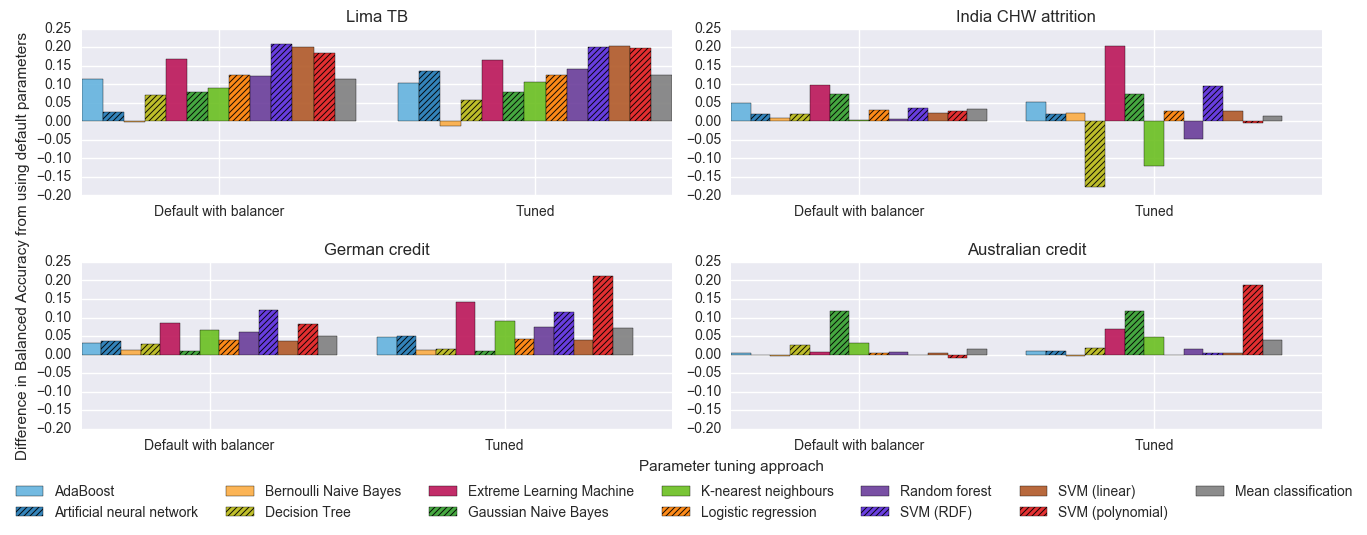
\includegraphics[scale=0.6]{Parameter_tuning_approach_results_per_classifier_plot_['Lima_TB',_'India_CHW_attrition',_'German_credit',_'Australian_credit']_Balanced_Accuracy_2016-10-30_18-02-09}}
		\caption{Difference in balanced accuracy from using default parameters with different parameter tuning approaches}
		\label{fig:parameter_tuning}
		\vspace{-1em}
	\end{figure*}
	
	We see the largest improvement in BACC on the Lima TB dataset, incorporating a data balancing technique greatly improves the BACC for all but one classifier. The exception is Bernoulli naive Bayes where there is no difference in BACC for each dataset. We could not find any literature to explain why no difference was seen. In addition, non of the parameters that were searched, affected the classification greatly.
	%TODO: Try find out why Bernoulli naive Bayes isn't different
	
	Note that ELM did not have default parameters so we set the default ELM to have one hidden layer with 100 neurons using the sigmoid activation function. We chose this as it is very similar to what scikit-learn \cite{scikit-learn} uses as its default parameters for the ANN.
	
	The CLC classifier was excluded as the classifier would crash when applied to the Lima TB dataset without any data balancing technique.
	
	Across all of our datasets, we see marginal improvements on average from tuning our classifiers. Typically the improvement is less than 0.05 from using the default parameters with a data balancer. On the Lima TB dataset the ANN sees an improvement of 0.1 with the tuned parameters over just using the default with a data balancer. On the other datasets we see large improvements for the ELM when tuned. Given that the architecture of a multi-layered perception such as an ANN or ELM  While the SVM with RBF and linear kernel see similar results between default with balancer and tuned, the SVM with polynomial kernel sees a large improvement on the credit scoring datasets when tuned.
	
	A classifier that has minor differences between default with balancer and tuned BACC across each dataset is preferred. It shows that the classifier will always produce the best results it can without the user having to manually identify the optimal parameters for each dataset or subset of a dataset that is used to answer a particular research question. LR, AdaBoost, RF, Bernoulli NB and SVM with RBF and linear kernel showed similar results between default with balancer and tuned across all our datasets. If these classifiers show promising classification results compared to the other classifiers then they will be recommended. We investigate that in Section \ref{classifier-results}.

	\subsection{Classifier results}
	\label{classifier-results}
	Table \ref{table-lima-tb-results} and \ref{table-india-attrition-results} contain the results for each classifier on the Lima TB and India attrition datasets respectively. SVM with linear and polynomial kernel saw very long training times when the ability to produce probabilistic output was enabled for the India attrition dataset. We disabled probabilistic output so results for BS and H-measure are unavailable for those classifiers. The CLC classifier does not support probabilistic output and therefore does not contain results for those metrics either. Figure \ref{fig:classifier_comparision} compares the difference in TPR and FPR from the median TPR and FPR calculated for every classifier on each dataset. Classifiers that consistently produce better than average results should be in the upper right quadrant. Classifiers in the upper left and lower right can produce better than average results if the improvement in either TPR or TNR exceeds that of the reduction in TNR or TPR. 
	
	For all our datasets, ANN and LR produce high quality classification. LR has two benefits over an ANN, it produces a white-box model that can be interpreted to understand the classification process \cite{Dreiseitl2002352} and its training time is orders of magnitude faster than an ANN. As the ANN can produce a non-linear model it should be able to produce results better than those that are limited to a linear model. However, our statistical tests indicate that that is no statistical difference between the BACC of the ANN and LR ($p=0.46$) across the datasets. It is possible that our datasets are too small and contain too few features to truly utilise the ANN to its full potential. 
	
	Bernoulli NB produced impressive results for the India attrition dataset showing no significant difference in BACC from the ANN ($p=1.0$). Bernoulli NB has the added benefit that it scales well with data size and number of features. The performance of Bernoulli NB is unexpected as it is designed to operate on binary features. For each dataset we already convert categorical features to multiple binary features as part of the one-hot encoding. However, Bernoulli NB has to apply binarizing on numerical features to transform them into binary features. This process could result in the loss of important information. Since our numerical features are scaled to that of a normal distribution, a binarization threshold of 0 is optimal where input greater than 0 becomes 1 and input lower becomes 0. On our attrition dataset which has 3840 entries per fold and 270 features, once pre-processing is completed, is able to fit a fold in 0.02 seconds. This is the fastest of all the classifiers for the particular dataset. In addition it showed the most stable results in our parameter tuning experiment indicating that minimal tuning is required. Bernoulli NB is therefore well suited for rapid experimentation and prototyping of ideas because of its fast training times and solid classification performance.

	The ELM showed BACC on par with SVM with RBF kernel ($p=0.99$) and ANN ($p=1.0$) on the two credit scoring datasets matching that of Huang \textit{et al.} \cite{6035797, Huang2006489}. However, on our TB and attrition dataset the ELM was significantly worse than that of the ANN ($p<0.01$) but obtained similar results to that of the SVM with RBF kernel ($p=1.0$). The ELM does deliver on its claim that it can learn significantly faster than an ANN. It is 13 times faster on the attrition dataset, 64 times faster on the TB dataset, 189 times faster on the German credit dataset and 802 times faster on the Australian credit scoring dataset.
	
	We were unable to replicate Luo \textit{et al.}'s \cite{Luo20097562} results for the CLC on the credit scoring datasets. We were only able to achieve a BACC of 0.6048 and 0.5744 on the German and Australian dataset respectively where Luo \textit{et al.} achieved an accuracy of 0.8480 and 0.8652. Since the Australian dataset is balanced, BACC is the same as accuracy. On the Lima TB dataset and India attrition dataset we were unable to achieve results better than random with the CLC classifier. Luo \textit{et al.}'s accuracy of 0.8480 on the German credit scoring dataset is far higher than that seen in the other credit scoring literature utilizing the dataset. The literature typically obtains an accuracy of 0.77 for the dataset \cite{Huang2007847, Nanni20093028, Tsai20082639, Wang2011223}. We tried a variety of different formatting for our datasets to ensure that we had it formatted correctly for the CLC classifier. We tested different values for the classification labels, different placement of the label either as the first column or last column in the dataset and the dataset formatted as either CSV or TSV. Our testing indicated that the classification label should be the first column and input formatted as a TSV file. The exact values of the labels was not found to be important for the classification Based on our observations, we would not recommend the use of CLC for future classification tasks.	
	
	Table \ref{table-dataset_signifigance} contains the $p$-values from the Nemenyi multiple comparison test with the best ranked classifier for each metric. We reject the null-hypothesis at a $p$-value $< 0.05$. The ANN, RF and LR show similar results across multiple metrics.
	
	
	\begin{table*}
		\centering
		\small
		\vspace{-3em}
		\caption{Lima TB metrics\textsuperscript{*} for each classifier}
		\label{table-lima-tb-results}	
		\vspace{-1em}
		\scalebox{0.9}{	
		\begin{tabular}{l|c|c|c|c|c|c|c} \hline		
			Classifier&BACC&MCC&BS&H-measure&TPR&TNR&\parbox[t]{1.1cm}{\centering Time to fit\textsuperscript{\textdagger} (s)}\\ \hline 
			ANN			&\textbf{0.7109 (0.0432)}	&0.3044 (0.0601)		&\textbf{0.1740 (0.0414)}	&0.3392 (0.0864)			&0.6434 (0.0918)				&0.7785 (0.0319)			&0.3552 (0.0547)\\  
			LR			&0.7103 (0.0438)			&0.3028 (0.0602)		&0.1743 (0.0120)			&0.3375	(0.0877)		&0.6439	(0.0943)			&0.7768	(0.0305)		&0.0058 (0.0004)\\ 
			SVM (linear)&0.7006 (0.0419)			&0.2969 (0.0569)		&n/a						&n/a			&0.6061	(0.0987)			&0.7951 (0.0374)			&0.2178	(0.0287)\\ 
			AdaBoost	&0.6998 (0.0453)			&0.2756 (0.0604)		&0.2411	(0.0019)			&\textbf{0.3493	(0.0867)}		&0.6683 (0.0975)				&0.7314	(0.0355)		&0.0870	(0.0440)\\ 
			Bernoulli NB&0.6966 (0.0471)			&0.2810 (0.0654)		&0.1887	(0.0187)			&0.3143	(0.0901)		&0.6270	(0.0978)			&0.7663	(0.0339)		&0.0007	(0.0001)\\ 
			RF			&0.6964 (0.0494)			&0.2843	(0.0705)		&0.1916	(0.0135)			&0.3165	(0.0865)		&0.6191	(0.1071)			&0.7737	(0.0457)		&0.0446	(0.0053)\\ 
			ELM			&0.6953 (0.0515)			&0.2811	(0.0714)		&0.1836	(0.0140)			&0.3130	(0.0843)		&0.6199	(0.1100)			&0.7707	(0.0401)		&0.0050	(0.0010)\\ 
			SVM (RDF)	&0.6952 (0.0441)			&0.2821	(0.0612)		&0.1944	(0.0139)			&0.3232	(0.0848)		&0.6195	(0.1060)			&0.7709	(0.0496)		&0.0114	(0.0007)\\ 
			SVM (poly)	&0.6948 (0.0501)			&\textbf{0.3054 (0.0738)}&n/a						&n/a			&0.5608	(0.1092)			&\textbf{0.8288	(0.0434)}		&0.0018	0.0001\\ 
			Gaussian NB	&0.6777 (0.0769)			&0.2561	(0.1078)		&0.3021	(0.1664)			&0.3022	(0.0889)		&\textbf{0.7002	(0.1422)}			&0.6551	(0.2359)		&0.0012	(0.0001)\\ 
			DT			&0.6606 (0.0599)			&0.2402	(0.0931)		&0.2164	(0.0217)			&0.2144	(0.1058)		&0.5507	(0.1290)			&0.7704	(0.0884)		&0.0005	(0.0001)\\ 
			$k$NN		&0.6592 (0.0478)			&0.2253	(0.0642)		&0.2260	(0.0129)			&0.2053	(0.0778)		&0.5673	(0.1071)			&0.7511	(0.0348)		&\textbf{0.0003	(0.0000)}\\ 
			CLC			&0.5196 (0.0789)			&0.0264	(0.1057)		&n/a						&n/a			&0.5428	(0.1592)			&0.4964	(0.1503)		&0.0695	(0.0060)\\                  
			\multicolumn{5}{l}{\textsuperscript{*}\footnotesize{\parbox[t]{7.9cm}{Standard deviation in brackets}}}\\
			\multicolumn{5}{l}{\textsuperscript{\textdagger}\footnotesize{\parbox[t]{7.9cm}{Time to fit individual fold}}}  		
		\end{tabular}}
	\end{table*}
	
	\begin{table*}
		\centering
		\small
		\vspace{-1em}
		\caption{India attrition metrics\textsuperscript{*} for each classifier}
		\label{table-india-attrition-results}	
		\vspace{-1em}
		\scalebox{0.9}{	
		\begin{tabular}{l|c|c|c|c|c|c|c} \hline		
			Classifier&BACC&MCC&BS&H-measure&TPR&TNR&\parbox[t]{1.1cm}{\centering Time to fit\textsuperscript{\textdagger} (s)}\\ \hline 
			Bernoulli NB&\textbf{0.8188 (0.0121)}	&0.6017	(0.0236)			&0.1526	(0.0087)			&\textbf{0.5312	(0.0275)}	&0.8789	(0.0167)			&0.7587	(0.0201)			&\textbf{0.0202	(0.0006)}\\ 
			ANN			&0.8182 (0.0138)			&\textbf{0.6123	(0.0280)}	&0.1363	(0.0101)			&0.5261	(0.0285)			&0.8208	(0.0278)			&0.8156	(0.0261)			&4.4187	(1.2427)\\  
			RF			&0.8118 (0.0135)			&0.6113	(0.0264)			&\textbf{0.1301 (0.0069)}	&0.5205	(0.0267)			&0.7758	(0.0232)			&0.8478	(0.0148)			&1.9288	(0.1000)\\ 
			AdaBoost	&0.8035 (0.0140)			&0.5989	(0.0273)			&0.1623	(0.0039)			&0.4882	(0.0294)			&0.7545	(0.0256)			&\textbf{0.8524	(0.0163)}	&6.5844	(0.2379)\\ 
			Gaussian NB	&0.8035 (0.0176)			&0.5800	(0.0367)			&0.2015	(0.0223)			&0.4304	(0.0470)			&0.8190	(0.0243)			&0.7879	(0.0356)&0.0255 (0.0042)\\ 
			LR			&0.8023 (0.0130)			&0.5689	(0.0248)			&0.1473	(0.0056)			&0.4977	(0.0245)			&0.8726	(0.0198)			&0.7320	(0.0192)			&0.4675	(0.0632)\\ 
			SVM (linear)&0.7968 (0.0137)			&0.5632	(0.0258)			&n/a					&n/a			&0.8275	(0.0270)			&0.7661	(0.0191)			&8.4384	(1.2798)\\ 
			DT			&0.7753 (0.0136)			&0.5321	(0.0271)			&0.1987	(0.0108)			&0.3876	(0.0305)			&0.7530	(0.0246)			&0.7977	(0.0210)			&0.2952	(0.0448)\\ 
			SVM (RBF)	&0.7726 (0.0135)			&0.5132	(0.0256)			&0.1658	(0.0076)			&0.4345	(0.0276)			&0.8399	(0.0320)			&0.7054	(0.0309)			&6.1570	(0.2249)\\ 
			ELM			&0.7694 (0.0146)			&0.5135	(0.0289)			&0.1577	(0.0072)			&0.4159	(0.0284)			&0.7778	(0.0242)			&0.7610	(0.0224)			&0.2982	(0.0089)\\ 
			$k$NN		&0.7651 (0.0152)			&0.5147	(0.0304)			&0.1599	(0.0090)			&0.3978	(0.0289)			&0.7298	0.0250)			&0.8004	0.0197)			&0.0660	(0.0078)\\ 
			SVM (poly)	&0.5247 (0.0064)			&0.1095	(0.0234)			&n/a			&n/a			&\textbf{0.9865	0.0068)}&0.0630	0.0115)			&1.5029	(0.0550)\\ 
			CLC			&0.5081 (0.0116)			&0.0361	(0.0451)			&n/a			&n/a			&0.6444	(0.4506)			&0.3718	(0.4461)			&2.3504	(0.3767)\\                  
			\multicolumn{5}{l}{\textsuperscript{*}\footnotesize{\parbox[t]{7.9cm}{Standard deviation in brackets}}}\\
			\multicolumn{5}{l}{\textsuperscript{\textdagger}\footnotesize{\parbox[t]{7.9cm}{Time to fit individual fold}}}
			  		
		\end{tabular}}
	\end{table*}

	\begin{table}
		\centering
		\vspace{-1em}
		\small
		\caption{Pairwise comparison using Nemenyi multiple comparison against best ranked classifier\textsuperscript{*} across all datasets\textsuperscript{\textdagger}}
		\label{table-dataset_signifigance}	
		\vspace{-1em}
		\hspace*{-2em}
		\scalebox{0.9}{	
			\begin{tabular}{l|c|c|c|c|c} \hline		
				Classifier&BACC&MCC&BS&H-measure&Time to fit\textsuperscript{\textdaggerdbl}\\ \hline
				ANN			&--					&--					&\textbf{1.0}	&--					&<0.0001\\ 
				Bernoulli NB&0.04842			&0.00563			&<0.0001		&0.00022			&\textbf{0.17008}\\  
				RF			&\textbf{0.31338}	&\textbf{0.98923}	&--				&\textbf{0.99999}	&<0.0001\\ 
				Gaussian NB	&<0.0001			&<0.0001			&<0.0001		&<0.0001			&0.02760\\ 
				AdaBoost	&<0.0001			&0.00036			&<0.0001		&0.00651			&<0.0001\\ 
				LR			&\textbf{0.46228}	&\textbf{0.08012}	&0.00530		&0.00237			&<0.0001\\ 
				SVM (linear)&0.00779			&\textbf{0.06460}	&n/a			&n/a				&<0.0001\\ 
				DT			&<0.0001			&<0.0001			&<0.0001		&<0.0001			&<0.0001\\ 
				SVM (RBF)	&<0.0001			&<0.0001			&<0.0001		&0.00037			&<0.0001\\ 
				ELM			&<0.0001			&<0.0001			&0.00085		&<0.0001			&<0.0001\\ 
				$k$NN		&<0.0001			&<0.0001			&<0.0001		&<0.0001			&--\\ 
				SVM (poly)	&<0.0001			&<0.0001			&n/a			&n/a				&<0.0001\\ 
				CLC			&<0.0001			&<0.0001			&n/a			&n/a				&<0.0001\\\hline
				Friedman	& $\chi^2_{11} = 22$\textsuperscript{\textdaggerdbl}& $\chi^2 (11) = 22$\textsuperscript{\textdaggerdbl}& $\chi^2_{11} = 22$\textsuperscript{\textdaggerdbl}& $\chi^2_{11} = 22$\textsuperscript{\textdaggerdbl}& $\chi^2_{11} = 22$\textsuperscript{\textdaggerdbl}
				\\\hline
				\multicolumn{6}{l}{\textsuperscript{*}\footnotesize{\parbox[t]{7.9cm}{Represented with a ``--''}}}\\
				\multicolumn{6}{l}{\textsuperscript{\textdagger}\footnotesize{\parbox[t]{7.9cm}{Displayed as $p$-value with values bolded if they are not significant at $p=0.05$}}}\\
				\multicolumn{6}{l}{\textsuperscript{\textdaggerdbl}\footnotesize{\parbox[t]{7.9cm}{Null hypothesis of Friedman test rejected $(p<0.0001)$}}}
				
				              		
		\end{tabular}}
		\vspace{-1em}
	\end{table}
	
	\begin{figure}
		\hspace*{1em}
		\centering
		\makebox[\linewidth]{
			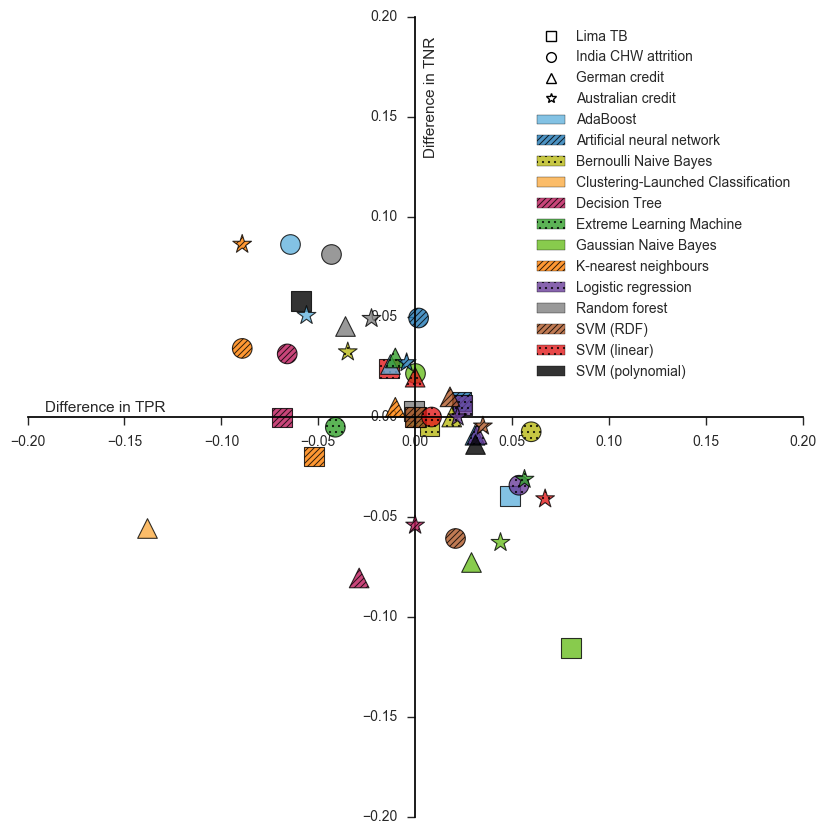
\includegraphics[scale=0.5]{classifier_dataset_plt_2016-11-07_14-58-15}}
		\caption{Difference from median TPR and TNR on each dataset for every classifier}
		\label{fig:classifier_comparision}
	\end{figure}
	
	\subsection{Data Balancing}
	Figure \ref{fig:classifier_vs_balancer} suggests that there is no clear winner among the data balancers. We average each balancer over the classifiers. ADASYN improves TPR for a minor reduction in TNR for the Lima TB dataset while EEN is able to improve the TPR for a minor reduction in TNR for the two credit scoring datasets.
	
	Unlike our classifiers, there is no clear-cut recommendations on which data balancers to use. For our credit scoring datasets, under-sampling techniques such as EEN and NCR produced the best results. For our Lima TB and India attrition dataset, oversampling techniques such as ADASYN produced the best results. SMOTETomek also performed well on the India attrition dataset.
	
	Our observations suggest that over-sampling techniques are best suited to datasets that have a higher imbalance ratio where under-sampling techniques are better suited to datasets that have a lower imbalance ratio. We suggest using one of ADASYN, SMOTETomek, EEN or NCR.

	\begin{figure}
		\hspace*{-6em}
		\centering
		\makebox[\linewidth]{
			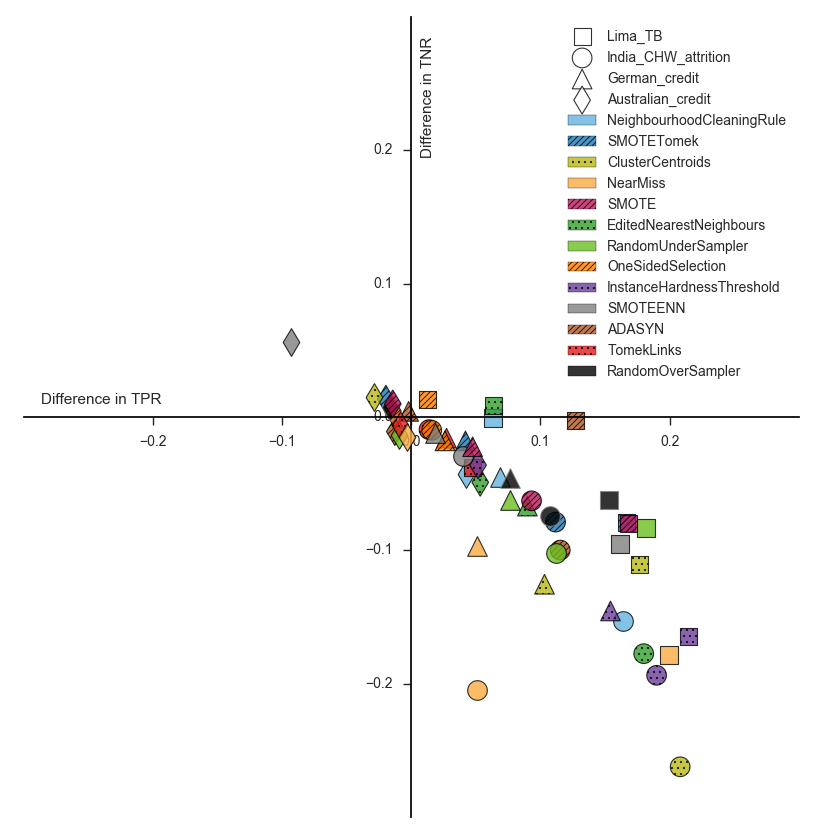
\includegraphics[scale=0.5]{classifier_dataset_plt_2016-11-08_02-09-25}}
		\caption{Difference from no balancer on each dataset for every balancing technique}
		\label{fig:balancing_per_dataset}
	\end{figure}
	\begin{figure*}
		\vspace{-5em}
		\centering
		\makebox[\linewidth]{
			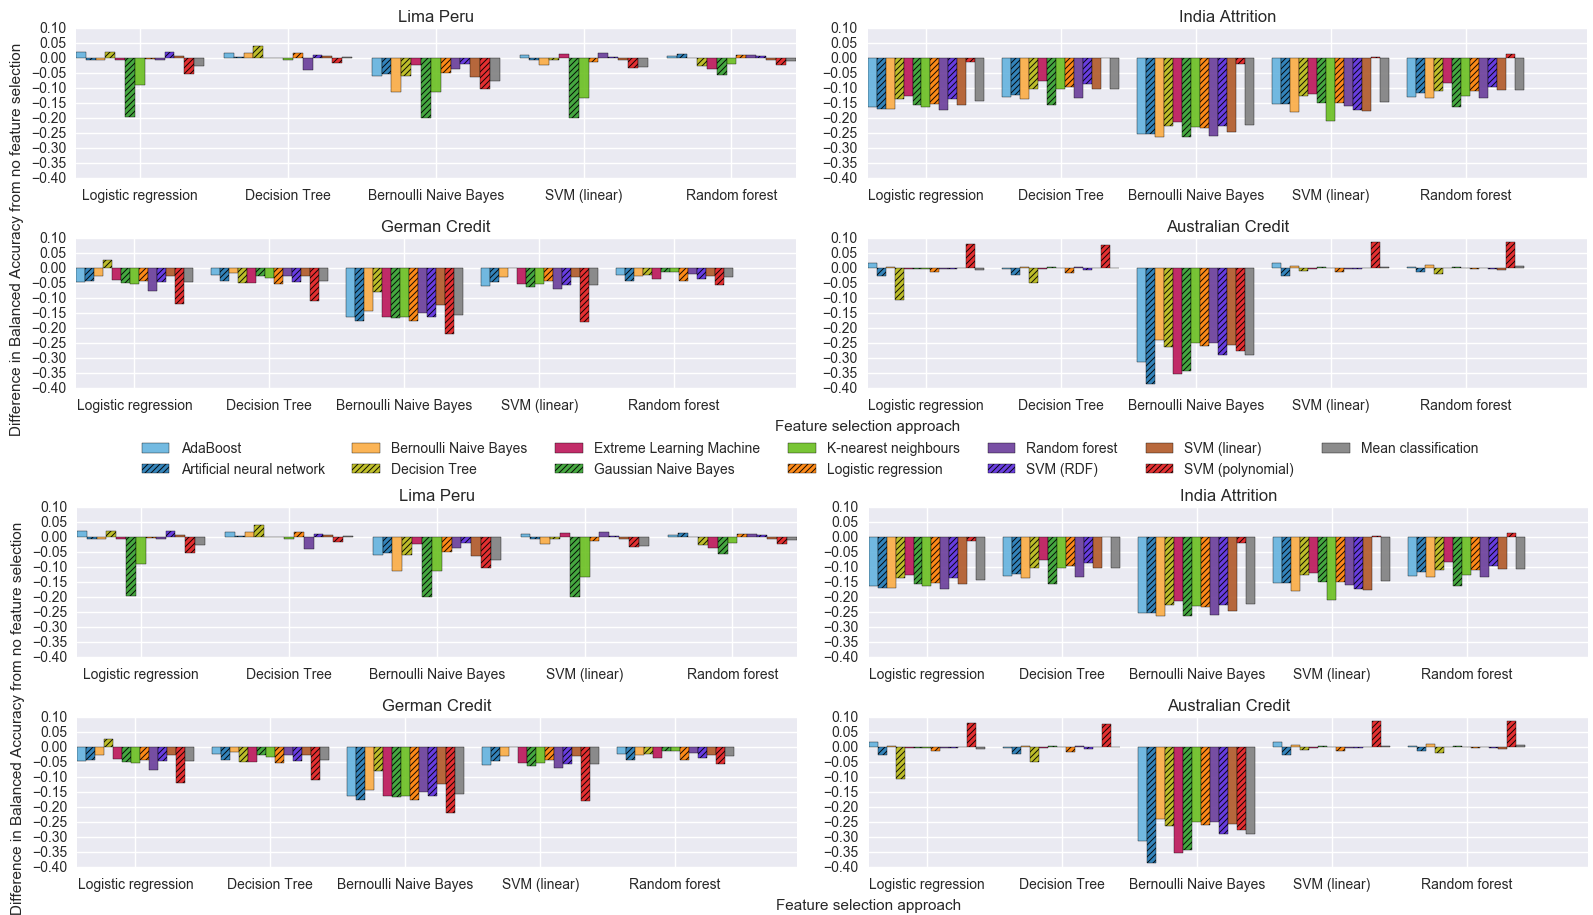
\includegraphics[scale=0.5]{feature_selection_edited_3}}
		\caption{Difference in BACC from using no feature selection with different feature selection approaches forced to select 15 features for each classifier (Top) and allowed to use any number of features (Bottom)}
		\label{fig:feature_selection_limit_15}
	\end{figure*}
	
	\subsection{Feature selection}
	Our feature selection experiment is divided into two sub-goals, identifying the most important predictors and removing un-important features. Figure \ref{fig:feature_selection_limit_15} contains the results for our first sub-goal. Across our datasets RF and decision tree were able to identify the most important features. Bernoulli BR is not recommended for selecting the most important features.
	
	Our second goal was to use feature selection to remove unnecessary features while maintaining overall BACC. Bernoulli Naive Bayes only removed a small subset of features from each dataset. SVM (linear) and RF were both able to reduce the number of features substantially while maintaining overall BACC. However, SVM (linear) reduced the number of features less that that of RF. On the India Attrition dataset the number of features were reduced from 272 to 204.8 and 191 on average for each training fold using SVM (linear) and RF respectively.
	
	We recommend the use of RF for both identifying the most important predictors and removing un-important features.
	

	
	\subsection{Analysis of time to default on Lima TB dataset}
	The only default range that showed a large variation in BACC from that of the others was training using the 300+ default range. Using this range resulted in a low TPR when applied to the testing set which contains the other half of non-defaulters and defaulters outside this default range. 
	
	Our analysis suggests that a defaulter's ``profile'' is similar for those who default within 300 days but different for those who default after.	
	
	\section{Conclusions and Future Work}
	While our comparison of classifiers, data balancers and features selection strategies is extensive we are limited by the datasets that were available to us for this study. The number of samples in our datasets are small compared to what is available in a production environment which limits our ability to see how our results scale to much larger datasets.
	
	Future work includes the use of datasets which are orders of magnitude larger and the incorporation of temporal data into TB default prediction. Temporal data could include information from each check-up to improve the prediction. Our TB default data only contained information available at registration.
	
	The use of data balancing techniques greatly improved BACC for our imbalanced datasets. Parameter tuning only resulted in marginal improvements for most classifiers. The ANN on the TB dataset and ELM on the other datasets saw the greatest improvement in BACC from parameter tuning.
	
	The use of LR, ANN, RF and Bernoulli NB are recommended for several reasons. Bernoulli NB showed above median performance and it can trained incredibly fast. This allows it to scale well for large datasets and facilitates rapid testing and improvement of one's experimental design. ANN produced excellent results in all our datasets and achieved the highest BACC, MCC and MCC across the datasets. LR produced good BACC and MCC in the Lima TB and German credit dataset. It also showed competitive performance in the other two datasets. LR produces a white-box model which allows for easier interpretation of the classification process. No statistical difference was found between RF and ANN across the datasets in any of the metrics.
	
	There was no stand-out data balancing algorithm. However, ADASYN was best on the Lima TB dataset and ENN was best on the two credit scoring datasets.
		
	Most of papers in Section \ref{predictors_of_defaulters_related_work} used LR to determine the predictors associated with TB default. Our results suggest that RF is better at identifying important predictors. Random forest also showed the best performance when RFE was applied. It was able to both reduce the number of features while retaining similar BACC and in some cases was able to improve the BACC too.
	%
	% The following two commands are all you need in the
	% initial runs of your .tex file to
	% produce the bibliography for the citations in your paper.
	\bibliographystyle{abbrv}
	\bibliography{sigproc}  % sigproc.bib is the name of the Bibliography in this case
	% You must have a proper ".bib" file
	%  and remember to run:
	% latex bibtex latex latex
	% to resolve all references
	%
	%\balancecolumns
\end{document}
